\subsection{IPS-N Blackbeard}

\begin{figure}
\begin{center}
    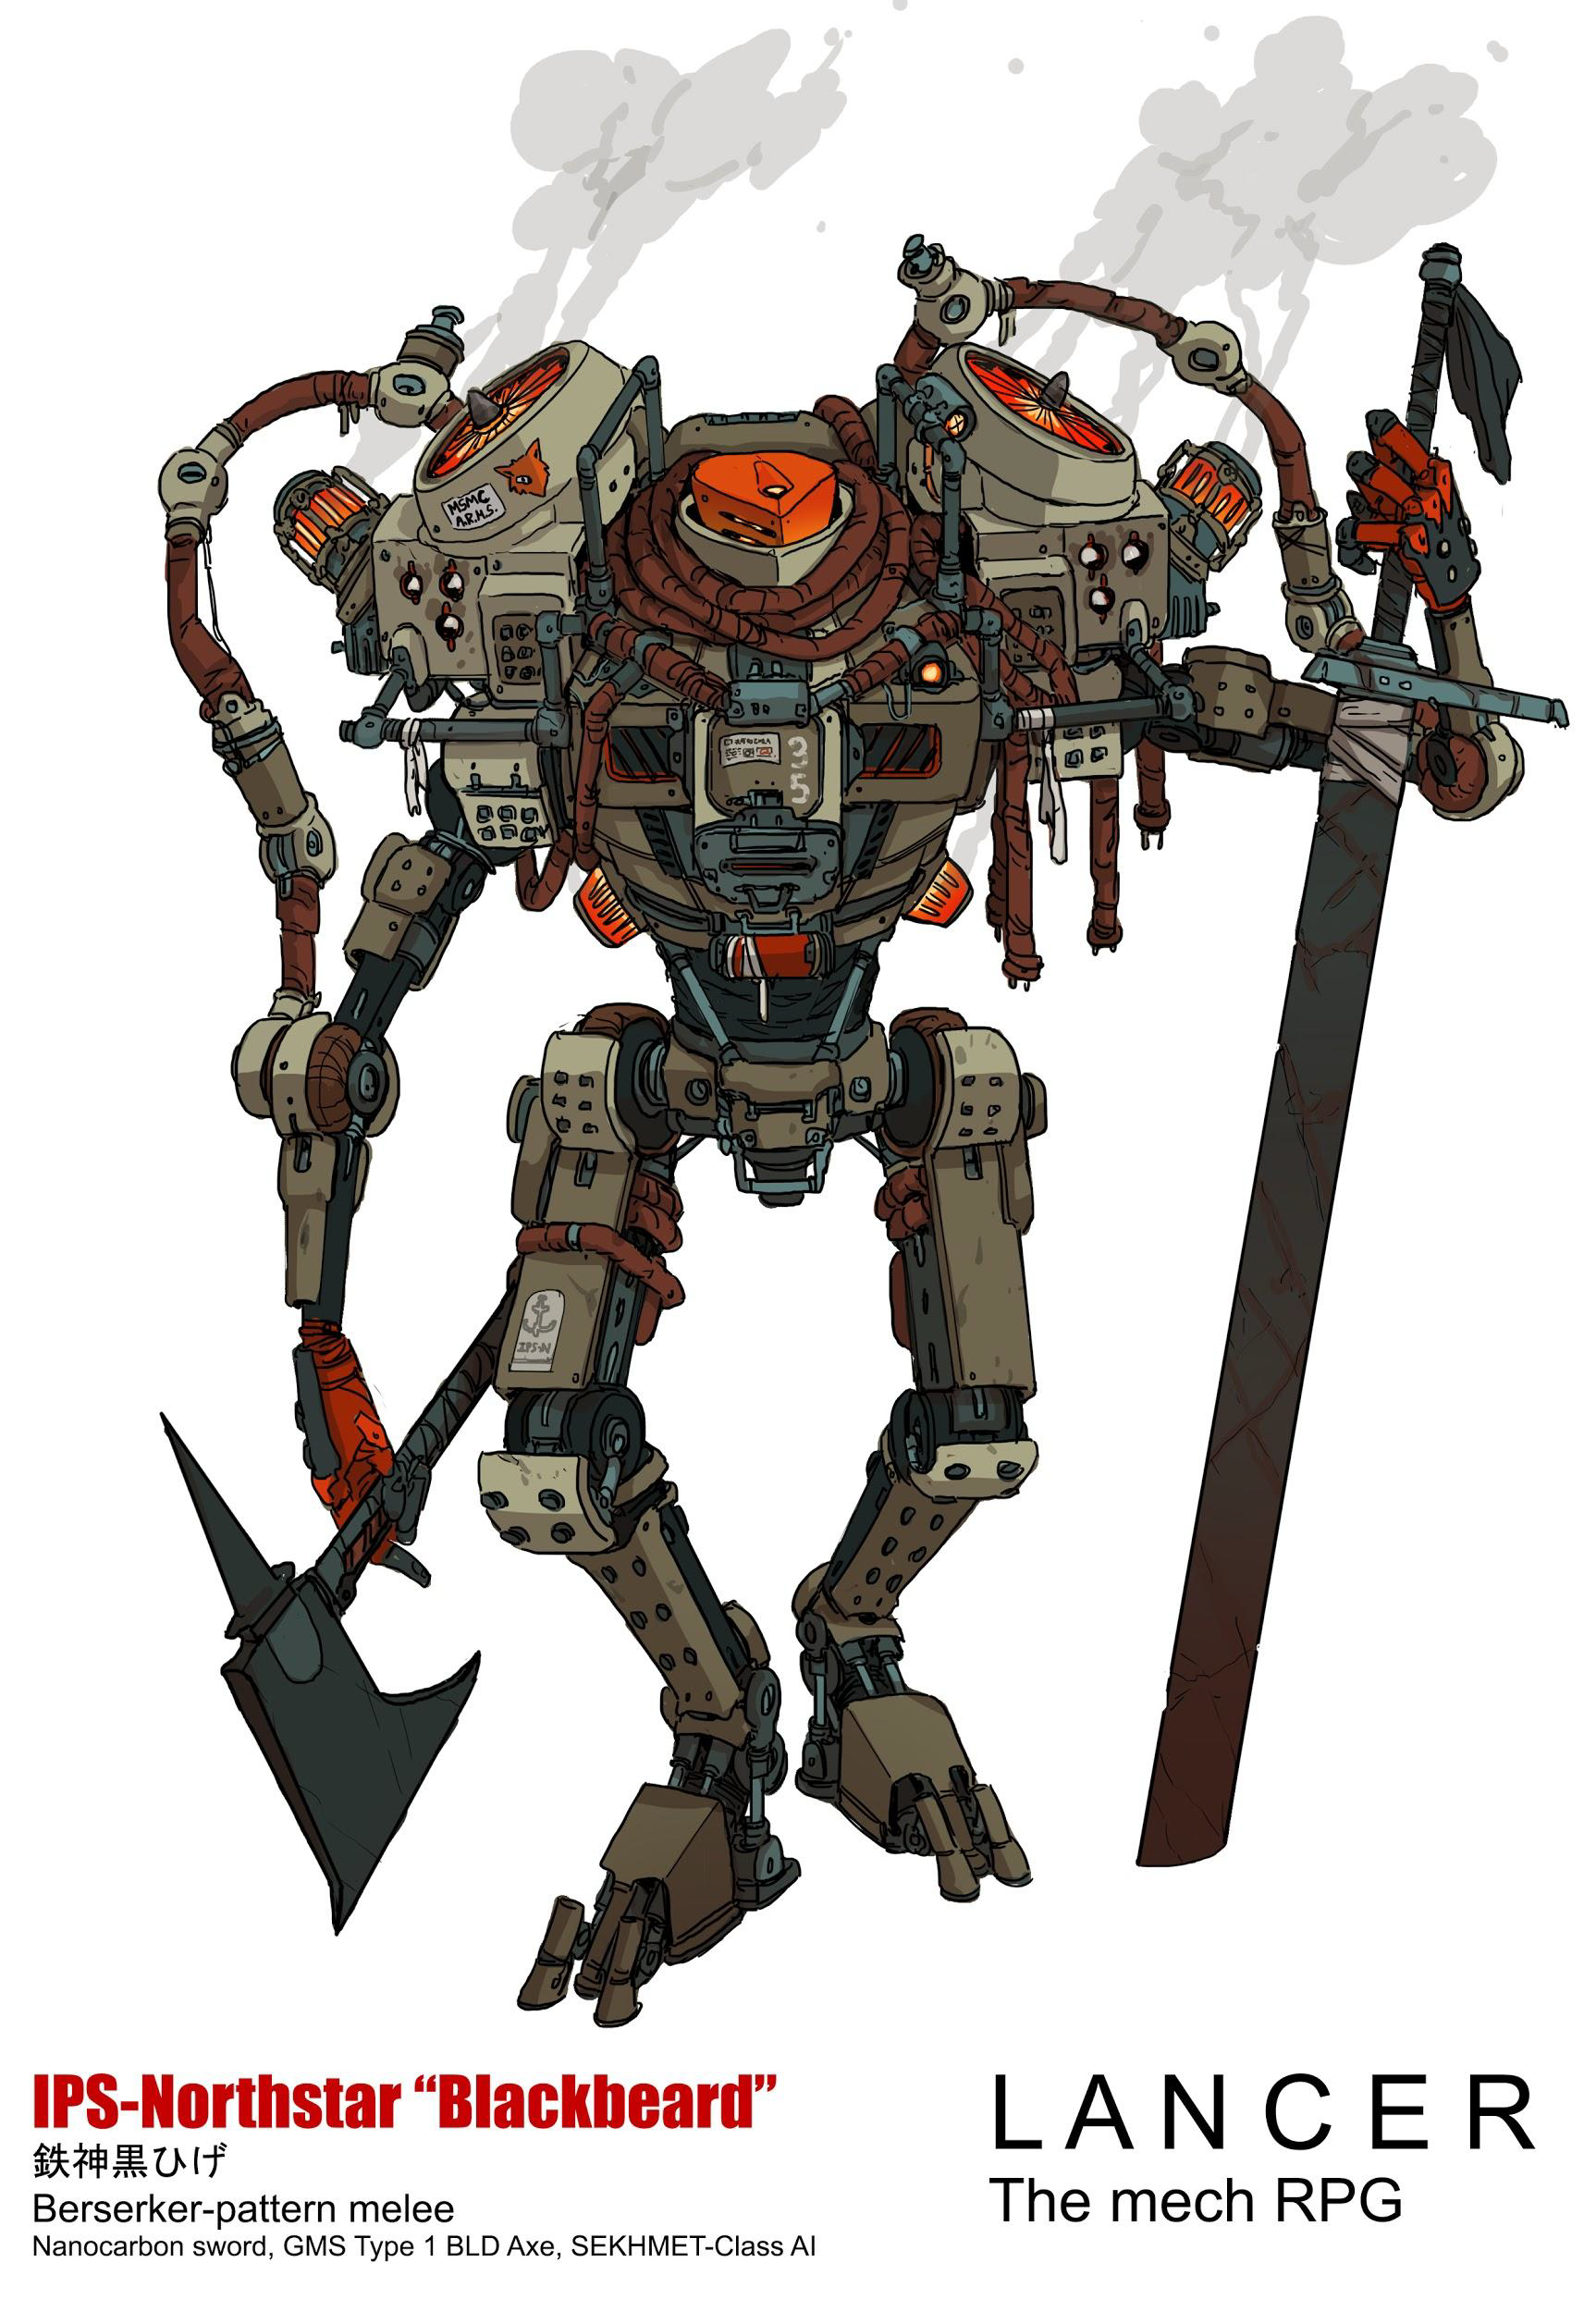
\includegraphics[width=\linewidth]{Blackbeard}
\end{center}
\end{figure}

\begin{mech}{IPS-N}{Blackbeard}

\fluff{The IPS-N BLACKBEARD is IPS-N’s solution for an aggressive, front-facing, preemptive anti-piracy platform. The BLACKBEARD license range is built for environments where combustible kinetic weaponry is either useless, too dangerous, or would prompt unnecessary collateral damage. Its distinctive, slim frame is a evocative of its speed and reduces its radar profile, making it hard to track and harder still to hit. The BLACKBEARD platform has been split into two model lines, the IPS-N/BB-L, which is the standard production line model, and the IPS-N/BB-Sk, a prototype limited print run of BB models purpose-built to contain IPS-N’s SEKHMET NHP platform.}

\begin{license}
\item Synthetic Muscle Netting, Chain Axe
\item BLACKBEARD FRAME, Flechette Launcher, Nanocarbon Sword
\item Reinforced Grapples, SEKHMET class NHP
\end{license}

\frameBox
[hp = 12,
evasion = 8,
speed = 5,
heat cap = 4,
sensors = 5,
armor = 1,
e-defense = 6,
size = 1,
repair cap = 4,
tech attack = -2,
traits = {\textbf{Cable Grapple:} The Blackbeard can initiate grapples up to range 5 away. If it successfully grapples its target, the Blackbeard is immediately pulled adjacent to its target by the straightest path possible (if it can’t move adjacent to its target, the grapple breaks).

\textbf{Lock/Kill Subsystem:} The Blackbeard can boost and take reactions while grappling.

\textbf{Exposed reactor:} The Blackbeard gets +1 Difficulty on engineering checks},
sp = 5,
mount one = flex mount,
mount two = main mount,
mount three = heavy mount,
core system name = Assault Grapples,
core system text = {The IPS-N branded assault grappling system is a proven, class-leading system rated to handle hauling, supporting, and securing chassis up to Galactic Standard Size 4. Grapple heads are interchangeable and can be swapped for hard or soft targets, electrified, or loaded with codespike systems to incapacitate targets at a distance.},
core active name = Omni-harpoon,
core active text = {Quick action

This one-shot system fires harpoon-like grapples at any number of targets within line of sight and within range 5. Those targets must pass a hull check with 1 difficulty or be knocked prone and pulled adjacent to your mech, or as far as possible towards your mech without being obstructed. All targets are then immobilized until the end of your next turn}]


Synthetic Muscle Netting
IPS-N’s proprietary Synthetic Muscle Netting is a field-proven augmentation compatible with existing IPS-N FRAMEs. A spray-on catalytic/structural enhancement, the SMN system boosts manipulator and propulsion subsystems by roughly 25\% without impacting the operational life of augmented components. The spray-on catalytic also acts as a mild impact-absorption and thermal insulation layer; IPS-N recommends pilots only apply the SMN system to interior components and practice frequent cleaning to prevent septic-analogous decay.

2 SP, Unique
When grappling or ramming, you always count as the same size as your opponent if your opponent is larger than you, and larger than your opponent if they are the same size or smaller. Your lifting and dragging capacity doubles.

Chain Axe
A simple tactical scale-up of a felling axe, IPS-N’s chain axe is a serrated, powered chainblade hardlinked to a chassis’ power core. The teeth of the IPS-N chain axe are tungsten-tipped, hardened to chew through hard and soft targets both. It is an effective weapon and utility tool, and is often used by boarding parties to make initial breaches in ship and station bulkheads.

Main Melee
Threat 1
Reliable 2
1d6 damage
On a critical hit, your target is Shredded until the end of your current turn

Nanocarbon Sword
IPS-N’s nanocarbon sword is a new spin on an old essential. Embedded nanosensors along the length of the blade capture a full spectrum of data while in use, recording to cloud-based Omninet storage banks for after-action review. Live feedback is relayed to the user, interpreted by their equipped sensor suite, and real-time adjustments are made to the molecular composition of the blade edge.

Heavy Melee
Reliable 3
Threat 2
1d6+4 kinetic damage

Flechette Launcher
The IPS-N Flechette Launcher utilizes a hive-analogous construction to project a total soft target kill zone in a dome around the user, denying personnel the opportunity to engage in aggressive infantry-tier actions.

Auxiliary CQB
Burst 1
1 Kinetic Damage
This weapon deals 3 damage instead of 1 against grappled targets or targets with the biological tag.

Reinforced Grapples
2 SP
Grapple movement: Once a turn, your mech can use this grapple when it makes a regular move, allowing it to Fly as long as it moves in a straight line and there is a clear path. It must end its move on an object or surface or fall, but can grab on to that surface (even vertical or overhanging) as long as it remains immobile. If it’s knocked prone or knocked back while grabbing onto a surface this way, it falls.
Drag Down: These grapples can also be used to target another actor within range 5 as a quick action. Make a contested hull check with your target. The loser is knocked prone.

SEKHMET-class NHP
The IPS-N SEKHMET Co-pilot is ready to be your First Mate! SEKHMET comes standard with remote, Omninet, IR tag, and voice control systems and is fully versed in all current and legacy IPS-N mech cores. Your own SEKHMET system will learn with you, and should the worst happen, will continue as you would, running an emulated neural net doppelgänger to control your IPS-N chassis until forced or voluntary shutdown.

SEKHMET-class systems tend to have aggressive attitudes and dark sense of humor; pilots often like to call them a berserker system, a dangerous NHP that values combat efficacy over its pilot’s well being.

3 SP, Unique
AI
Your mech gains the AI property. In addition, gain the SEKHMET protocol:

SEKHMET protocol
Protocol
All melee Critical Hits do an additional +1d6 bonus damage
You can make a skirmish action using only melee weapons as a Free Action at any point during your turn.

While active, you lose direct control of your mech. Your mech uses all available actions and movement to first attempt to get into melee range of the closest target (friend or foe!) and then attack them using all weapons. If your mech isn’t in melee range of a target, it attempts to use all actions to get into melee range, even if it could still fire a ranged weapon using those actions. You can decide to overcharge your mech or not, but if you do, it uses the overcharge action for the same purposes.

To end this protocol, you must pass a successful engineering check at the start of your turn. Otherwise, this protocol will continue until your mech is destroyed. Death or incapacitation of the pilot will not stop it.


\end{mech}
